\section{Preliminaries}\label{sec:preliminaries}

We write $2^S$ for the set of all subsets, i.e., the power set, of a set $S$. If a function $f : A \to B$ and $S \subseteq A$, we let $f(S) = \set{ f(a) : a \in S }$. For a set of sets $S$, we write $\cup S = \bigcup_{x \in S} x$.  If $f : A \to T$, where $T$ is a set, and $S \subseteq A$, we let $f(S) = \bigcup_{x \in S} f(x)$.

\subsection{Conjunctive Queries and Hypergraphs}

Conjunctive queries can be represented by hypergraphs, and our terminology follows the seminal references on this topic~\cite{DBLP:journals/jcss/GottlobLS02,DBLP:journals/jcss/GottlobLS03,DBLP:conf/wg/GottlobGMSS05,DBLP:conf/pods/GottlobGLS16,wang_yannakakis_2025}.
Let $\mathcal{D} = \{R_1[\bar{x}_1], \cdots, R_n[\bar{x}_n]\}$ be a database consisting of $n$ relations, where $\bar{x}_i$ is the set of attributes of relation $R_i$. A conjunctive query (with self-predicates) is defined as 
\[
    Q \gets \pi_{\bar{y}}\left(\sigma_{1}(R_1[\bar{x}_1]) \Join \cdots \Join \sigma_{n}(R_n[\bar{x}_n]\right)),
\]
where $\sigma_{i}$ is the set of selection predicates involving only attributes in $\bar{x}_i$, $\bar{y}$ is the set of output attributes, and $\Join$ denotes natural join (with attribute renaming to avoid ambiguity). If $\bar{y} = \bigcup_{i \in [n]} \bar{x}_i$, the query is called a full join query and we omit $\bar{y}$ for simplicity; if $\bar{y} = \emptyset$, the query is a Boolean query that returns true if there exists a tuple satisfying all specified joins and predicates, or false otherwise.  We also require the query to be \emph{self-join-free} at the logical level:  If multiple relations correspond to the same physical relation, they are treated as distinct logical relations with unique~renamings.

We define the associated \emph{hypergraph} for the conjunctive query $Q$ as $H=(V(H), E(H))$, where the vertices set $V(H)$ consists of all attributes appearing in the query, i.e., $V(H) = \bigcup_{i \in [n]} \bar{x}_i$, and the \emph{hyperedges} set $E(H) \subseteq 2^{V(H)} \setminus \set{ \emptyset }$ contains one hyperedge for each relation, i.e., $E(H) = \{e_1, \cdots, e_n\}$, where each $e_i = \bar{x}_i$.  

% The \emph{primal graph} of a hypergraph $H$ is the \emph{graph} on $V(H)$ which is obtained from $H$ by turning each hyperedge of $H$ into a clique. A hypergraph is connected if its primal graph is connected.  \emph{All hypergraphs in this paper are assumed to be finite, connected, and to have a non-empty set of hyperedges.}




%%%%%%%%%%%%%%%%%%%%%%%%%%%%%%%%%%%%%%%%%%%%%%
\subsection{Acyclicity and Join Trees}

A conjunctive query is acyclic if its associated hypergraph is acyclic, and we define acyclicity in the standard way in database theory, e.g.,~\cite[Section 6.4]{abiteboul_foundations_1996}. Namely, a hypergraph $H$ is acyclic if and only if the output of the GYO algorithm~\cite{grahamGYO, DBLP:conf/compsac/YuO79} on $H$ is empty~\cite[Theorem 6.4.5]{abiteboul_foundations_1996}. Equivalently, $H$ is acyclic if and only if there exists a \emph{join tree} \cite[Theorem 6.4.5]{abiteboul_foundations_1996}, or, a width-1 hypertree decomposition~\cite{DBLP:journals/jcss/GottlobLS02}.

Slightly differently from the usual definition of join trees~\cite{abiteboul_foundations_1996}, where each vertex is simply a relation, in this paper, we define them using notations for hypertree decompositions~\cite{DBLP:journals/jcss/GottlobLS02}, to make it easier to generalize to the meta-decompositions that we will define later.

Let $Q$ be an acyclic query with associated hypergraph $H$. A \emph{join tree} of $Q$ is a labeled tree $T = (V(T), r(T), E(T), \chi, \lambda)$
 with vertices $V(T)$, root $r(T)$, and edges $E(T)$.
$\chi : V(T) \to 2^{V(H)}$ is a function s.t.\ 
$\bigcup_{ p \in V(T) } \chi(p) = V(H)$,
and $\lambda : V(T) \to 2^{E(H)}$.\footnote{For simplicity, we may use hyperedges (e.g., $R_1$) to label and identify the vertices of join trees instead of writing the full $\lambda$- and $\chi$-labels when the context is clear.} And $T$ needs to satisfy the following~ conditions:
\begin{enumerate}[label=(C\textsubscript{\arabic*}),ref=(C\textsubscript{\arabic*}),leftmargin=*]
	\item\label{H1}\gdef\Giref{\ref{H1}} \textbf{Coverage condition.}  For each $e \in E(H)$, there exists exactly one $p \in V(T)$ with $\lambda(p) = \set{e}$.
	\item\label{H2}\gdef\Giiref{\ref{H2}} \textbf{Connectedness condition.} For each $v \in V(H)$, the set of vertices $\set{ p \in V(T) : v \in \chi(p) }$ induces a connected subtree of $T$.
    Or, equivalently, for all pairs of vertices $p, q \in V(T)$ and all $s$ on the (unique) path between $p$ and $q$ on $T$, we have $\chi(p) \cap \chi(q) \subseteq \chi(s)$.
	\item\label{H3}\gdef\Giiiref{\ref{H3}} \textbf{Width-1.} For all $p \in V(T)$, $|\lambda(p)| = 1$ and, without loss of generality, $\chi(p) = V(\lambda(p)) $.
\end{enumerate}

\begin{example}
    We revisit the query $Q_{\ref{ex:123-12-13-23-intro}}$ in \cref{ex:123-12-13-23-intro}. Its hypergraph is illustrated in \cref{fig:123-12-13-23-hg}. It is easy to verify that the join tree in \cref{fig:123-12-13-23-meta} satisfies conditions \ref{H1} and \ref{H3}. Regarding condition \ref{H2}, consider, e.g., attribute \( x_1 \). The vertices in the join tree that include \( x_1 \) are the ones with \( R_1 \), \( R_2 \), and \( R_3 \), which induce a connected subtree. Similar arguments apply for all other attributes as well.
\end{example}

We assume all trees are rooted and consider rerootings as distinct trees.
We write $T_p$ as the subtree rooted at $p$, i.e., with $p$ and all its descendants. For every neighbor (child or parent) $q$ of vertex $p$ in $T$, we write $T_{p \to q}$ for the subtree with
\[
    V( T_{p \to q} ) = 
    \set{ s \in V(T) \setminus \{ p \} : \text{the path from } p \text{ to } s \text{ in } T \text{ contains } q }\text.
\]
Intuitively, if $q$ is a child of $p$, it is the same as $T_q$. If $q$ is a parent of $p$, it denotes the subtree of $T$ with all vertices except those in $T_p$.

We define the \emph{fan-out} $f(p)$ of any $p \in V(T)$ as 
% \[
	% f(p) = \begin{cases}\mathsf{deg}(p) - 1, & \text{if $p$ is not the root} \\ \mathsf{deg}(p), & \text{if $p$ is the root} \end{cases}
% \]
% where $\mathsf{deg}(p)$ is the degree (number of neighbours) of node $p$, and $f(p)$ corresponds to 
the number of children of $p$ on $T$.  The \emph{fan-out} of the entire tree $T$, denoted by $f(T)$, is the maximum fan-out among all nodes of $T$.
% \[
	% f(T) = \max_{p \in V(T)} f(p).
% \]

Given a join tree $T$, for every $p \in V(T)$, we define the \emph{induced query} $Q(p)$ as the join of all relations in the subtree rooted at $p$. 
% \[
%     Q(p) = \left\{\begin{array}{cl}
%         p & \text{if $p$ is a leaf node} \\
%         p \Join \left(\Join_{\text{$c$ is a child node of $p$}} Q(c)\right) & \text{Otherwise.}
%     \end{array}\right.
% \]

One important observation is that \emph{an acyclic conjunctive query may have an exponential number of distinct join trees}.

\begin{theorem}
    \label{thm:exp-join-trees}
    Consider \emph{star queries}\footnote{We note that, in some literature, e.g.,~\cite{birler_optimizing_2025}, such queries are called ``\emph{clique}'' queries, because their \emph{query graphs} are cliques. 
    % Regardless, it has been shown that optimizing such queries exactly is \NP-hard and takes exponential time~\cite{birler_optimizing_2025,scheufele_constructing_1996} (unless $\P = \NP$).
    }
    of the form
    \[
        Q_{\rm star} \gets R_1[\bar{x}_1] \Join \cdots \Join R_n[\bar{x}_n], 
    \]
    where for any $i, j \in [n]$, $\bar{x}_i \cap \bar{x}_j = \set{x}$, for some attribute $x$.  There are $n^{n-1}$ possible join trees for such a star query with $n$ relations. 
\end{theorem}

\begin{example}
    \label{ex:star}
    The query $Q_{\ref{ex:star}} \gets R_1[x_1, x_2] \bowtie R_2[x_1, x_3] \bowtie R_3[x_1, x_4] \bowtie R_4[x_1, x_5]$ is such a star query. \cref{fig:star-hg} shows its associated hypergraph, and \cref{fig:star-jts} shows two of its valid join trees.
    \begin{figure}
    \centering
    \begin{subfigure}{.49\linewidth}
        \centering
        \vspace{-\baselineskip}
        \begin{tikzpicture}[hypergraph,xscale=.8,yscale=0.8,trim left=0cm,trim right=0cm]
            \node[vertex,label={east:$x_1$}] (x1) at (0, 0) {};
            \node[vertex,label={east:$x_2$}] (x2) at (-1, 1) {};
            \node[vertex,label={east:$x_3$}] (x3) at (-1, -1) {};
            \node[vertex,label={west:$x_4$}] (x4) at (1, -1) {};
            \node[vertex,label={west:$x_5$}] (x5) at (1, 1) {};
        
            \begin{scope}[on background layer]
                
                \newcommand*{\pathri}{($(x2) + (-0.25,0.25)$)
                    to[out=45,in=45] ($(x1) + (0.25,-0.25)$)
                    to[out=-135,in=-135] ($(x2) + (-0.25,0.25)$)}
                    
                \newcommand*{\pathrii}{	($(x1) + (0.25,0.25)$)
                    to[out=135,in=135] ($(x3) + (-0.25,-0.25)$)
                    to[out=-45,in=-45] ($(x1) + (0.25,0.25)$)}
                
                \newcommand*{\pathriii}{($(x1) + (-0.25,0.25)$)
                    to[out=45,in=45] ($(x4) + (0.25,-0.25)$)
                    to[out=-135,in=-135] ($(x1) + (-0.25,0.25)$)}

                \newcommand*{\pathriv}{	($(x5) + (0.25,0.25)$)
                    to[out=135,in=135] ($(x1) + (-0.25,-0.25)$)
                    to[out=-45,in=-45] ($(x5) + (0.25,0.25)$)}
                
                \draw[hyperedge,looseness=1,draw=Red,fill=Red,fill opacity=.1] \pathri;
                \draw[hyperedge,looseness=1,draw=Fuchsia,fill=Fuchsia,fill opacity=.1] \pathrii;
                \draw[hyperedge,looseness=1,draw=NavyBlue,fill=NavyBlue,fill opacity=.1] \pathriii;
                \draw[hyperedge,looseness=1, draw=BurntOrange,fill=BurntOrange,fill opacity=.1] \pathriv;
        
                \node[text=Red] at (-1.75,1) {$R_1$};
                \node[text=Fuchsia] at (-1.75,-1) {$R_2$};
                \node[text=Cyan] at (1.75,-1) {$R_3$};
                \node[text=BurntOrange] at (1.75,1) {$R_4$};
                
            \end{scope}
        \end{tikzpicture}
        \vspace{-0.5\baselineskip}
        \caption{Hypergraph of the query}
        \label{fig:star-hg}
    \end{subfigure}
    \hfill
    \begin{subfigure}{.49\linewidth}
        \small
        \centering
        \hfill
        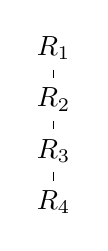
\begin{tikzpicture}[
			level distance=0.65cm,
			level 1/.style={sibling distance=1.2cm},
        ]
			\node { $R_1$ }
				child { node {$R_2$} edge from parent[-]
                    child { node {$R_3$} edge from parent[-]
                        child { node {$R_4$} edge from parent[-] }
                    } 
                };
		\end{tikzpicture}
        \hfill
        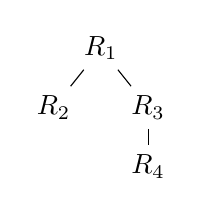
\begin{tikzpicture}[
			level distance=0.75cm,
			level 1/.style={sibling distance=1.2cm},
        ]
			\node { $R_1$ }
				child { node {$R_2$} edge from parent[-]
                }
                child { node {$R_3$} edge from parent[-]
                    child { node {$R_4$} edge from parent[-] }
                } ;
		\end{tikzpicture}
        \hfill
        \ 
        \caption{Two valid join trees}
        \label{fig:star-jts}
    \end{subfigure}
    \vspace{-0.5\baselineskip}
    \caption{Hypergraph and two valid join trees of the star query $Q_{\ref{ex:star}}$ in \cref{ex:star}}
    \label{fig:star}
\end{figure}


\end{example}

In fact, the possible join trees of such queries in \cref{thm:exp-join-trees} and \cref{ex:star} are simply \emph{all possible trees with $n$ vertices} (or, equivalently, all spanning trees of a complete graph $K_n$), each labeled by one relation. Any such tree satisfies the connectedness condition~\ref{H2}. 
There are a total of $n^{n-1}$ such trees ($n^{n-2}$ distinct non-rooted trees~\cite{prufer_neuer_1918}, each of which has $n$ possible root nodes).
% Each such tree can be encoded by a \emph{\prufer{} sequence}~\cite{prufer_neuer_1918} of length $n-2$ (where each element in the sequence can take values between $1$ and $n$ for a tree with $n$ vertices), plus one extra indicator for the root node.
% This gives a way to enumerate such trees without repetition.



\subsection{Query Plans and Join Ordering}
\label{sec:prelim-plans}

A \emph{query plan} $\mathcal{P} = (V(\mathcal{P}), r(\mathcal{P}), E(\mathcal{P}))$ for a query $Q$ is a tree rooted at $r(\mathcal{P})$, where each non-leaf node is a relational operator (e.g., join, projection, selection), and each leaf node corresponds to a base relation. 
% Since the query is self-join-free, every leaf node is distinct.  
A plan specifies an order of operations to evaluate the query, where the outputs of child nodes serve as inputs to the parent.
In this work, we focus on query optimization for binary joins, where each join operation in the query plan has exactly two child nodes.  
For the purpose of join ordering, \emph{we use only join operators in internal nodes and assume selections and projections are inherently integrated in the join
or scan
operation at the lowest possible level.}
Namely, in each step of join or scan, we apply a filter condition if all relevant attributes already appear in the subtree, and we project out attributes that neither appear in the output nor act as a join key with some remaining relation.

Given a query plan $\mathcal{P}$, for every $p \in V(\mathcal{P})$, we define the \emph{induced query} $Q(p)$ as the join of all relations in the subtree rooted at $p$ (with all possible projection and filters inherently applied).
% \[
%     Q(p) = \left\{\begin{array}{ll}
%         p & \text{if $p$ is a leaf node,} \\
%         % Q(c_1) & \text{if $p$ is unary operation,}\\
%         Q(c_1) \Join Q(c_2) & \text{if $p$ is join operation.}
%     \end{array}\right.
% \]

We exclude Cartesian products: for every join node, the outputs of its children must share some common attribute as the join key.
% with two child nodes $c_1$ and $c_2$, inducing subqueries $Q(c_1)$ and $Q(c_2)$, with output attributes $\bar{y}_1$ and $\bar{y}_2$, respectively, we require $\bar{y}_1 \cap \bar{y}_2 \neq \emptyset$.

A query plan is called \emph{left-deep} (or \emph{right-deep}) if all join operations have their right (left) child node corresponding to a base relation; otherwise, the query plan is referred to as \emph{bushy}.  
% , or unary operations applying to a base relation


We apply cost functions $\mathcal{C}$ on query plans, in the following form, to measure the optimality of query plans.
\[
    \mathcal{C}(\mathcal{P})= \left\{ \begin{array}{ll}
        c(r(\mathcal{P})), & \text{if $r(\mathcal{P})$ is single relation} \\
        % c(r)\oplus \mathcal{C}(\mathcal{P}_1), & \text{if $r$ is unary operation} \\
        c(r(\mathcal{P}))\oplus \mathcal{C}(\mathcal{P}_1) \oplus \mathcal{C}(\mathcal{P}_2), & \text{if $r(\mathcal{P})$ is join operation}
    \end{array} 
    \right.
\]
where $c(r(\mathcal{P}))$ is the cardinality of the output of $r(\mathcal{P})$; $\mathcal{P}_1$ and $\mathcal{P}_2$ (if applicable) are the left and right subtrees of $r(\mathcal{P})$, respectively; and $\oplus$ is some operator to aggregate $c(r)$, $\mathcal{C}(\mathcal{P}_1)$, and $\mathcal{C}(\mathcal{P}_2)$.  In this work, we adopt the cost function $C_{\rm out}$ to minimize the total intermediate result size by substituting the $\oplus$ operator simply with arithmetic $+$, as is standard in, e.g., \cite{stoian_dpconv_2024,fegaras_new_1998,neumann_adaptive_2018,cluet_complexity_1995}.  

The typical approach to find the optimal plan is to recursively find the optimal split of a set of relations into two disjoint subsets~\cite{selinger_access_1979,vance_rapid_1996,vance_join-order_1998,moerkotte_dynamic_2008,stoian_dpconv_2024}.   With a given cost function $\mathcal{C}$, the problem can be solved by the dynamic programming~(DP) algorithm DPccp~\cite{moerkotte_dynamic_2008} in $O(3^n)$. The recently proposed algorithm DPconv~\cite{stoian_dpconv_2024} reduces the complexity for the cost model $C_{\rm out}$ to $O(2^n n^3 W \log (Wn))$, where $W$ is the largest join cardinality.

